\chapter{Objectives Specification and Work Environment}

\section*{Introduction}
This chapter will first define the project's functional and non-functional requirements, then we will discuss the chosen structural deceisions , explaining the reasoning behind their selection. Finally we will specify the hardware and software resources necessary for this project. 

\section{Project Specification}
Requirements analysis is a fundamental phase in every project realization process. It is based on the study of the project's features as well as the constraints. In this section, we will cover both the functional and non-functional requirements.

\subsection{Functional Requirements}

The goal of the project is to generate a running CoreMark project on STM32 devices using CMSIS-Toolbox in an automated way. Within this context, this means guaranteeing the following concepts:

%\begin{itemize}
%    \item \textbf{Automation:} Ensuring that the user can generate a ready-to-build project without manually setting up peripheral configurations or memory layouts.
%    \item \textbf{Device Adaptability:} The project template must be dynamic in order to accomodate for the device specific characteristics of STM32 MCUs.
%    \item \textbf{CoreMark Integration:} CoreMark must be pre-configured and integrated within the project so that it can be executed immediately without further setup.
%    \item \textbf{Result Reporting:} The CoreMark results must be ouput in a standardized format, enabling consistent performance comparisons between devices.
%    \item \textbf{Multi-Toolchain Support:} The user should be able to build the project using any of the main embedded systems compilers without any extra configuration steps.
%\end{itemize}
%
%Table \ref{tab:functional_requirements} neatly summarizes the functional requirements for our project.

\begin{table}[htbp]
    \centering
    \caption{Functional Requirements for CMSIS-Toolbox based automated benchmarking}
    \label{tab:functional_requirements}
    \begin{tabularx}{\linewidth}{@{}>{\bfseries}l X X@{}}
        \toprule
        Requirements & Description \\
        \midrule
        Automation & The system must automatically generate a CoreMark benchmarking project for STM32 devices without requiring manual configuration. \\ \midrule
        Device Adaptability & The generated project must adapt to different STM32 families and configurations. \\ \midrule
        CoreMark Integration & The CoreMark benchmark must be integrated and ready to run immediately on the target hardware. \\ \midrule
        Result Reporting & The system must provide a standardized mechanism for reporting benchmark results. \\ \midrule
        Multi-Toolchain Support & The project must support multiple compilers such as GCC, ARM Compiler, and IAR. \\ \bottomrule
    \end{tabularx}
\end{table}
\subsection{Non-Functional Requirements}
Below are the non-functional requirements or the constraints that the functional expectations must abide by:
\begin{itemize}
    \item \textbf{Performance Requirements:}
    \begin{itemize}
        \item \textbf{Low Overhead} The project must not add significant, if any overhead besides the CoreMark runtime, this insures the integrity of the benchmarking results.
        \item \textbf{Compiler Optimizations} The project must provide the most optimal compiler configuration to ensure the maxmium performance results.
    \end{itemize}
   \item \textbf{Reliability Requirements:}
   \begin{itemize}
    \item \textbf{Correctness} The project must be functional and able to run without manual fixes.
    \item \textbf{Consistency} The project must produce consistent results amongst STM32 devices.
    \item \textbf{Error Handling} The project must fail gracefully and generate meaningful error messages.
   \end{itemize}
   \item \textbf{Usability Requirements:}
   \begin{itemize}
    \item \textbf{Ease of use} The generation process must be simple and intuitive, the project structure must be clear and consistent.
    \item \textbf{Standardized Output} The results must be presented in a clear format to facilitate further automation and data collection.
   \end{itemize}
\end{itemize}
\newpage

\section{Structural Decisions}
Before delving further into the implementation details, it is crucial to understand the rationale behind the structural decisions chosen, for both the generation tool and the CoreMark project. This sections elucidates the reasons behind the choices and their relevence to the project's objectives.
\subsection{CoreMark Project}
The CoreMark project is the end result of the generation tool, it is meant to be runnable out of the box with the 3 main compilers (GCC, ARM, and IAR).
For this reason, the following elements are provided:
\begin{table}[htbp]
   \centering 
   \caption{CoreMark Project Structure}
   \begin{tabularx}{\linewidth}{@{}>{\bfseries}l X X@{}}
    \toprule
    Element & Description \\
    \midrule
    User Code & This component provides the definition for the user application's entry point (the main() function) as well as the UART peripheral configuration. \\
    \midrule
    Driver & This component includes the necessary HAL drivers to enable the UART peripheral. \\
    \midrule
    Modifiable & This component contains the source and header files to modify if the user wants to modify system configurations such as linker files, startup code and VTOR configuration. \\
    \midrule
    CoreMark & This component contains the source code of the CoreMark benchmark to be invoked within the usercode's entry point. \\
    \midrule
    coremark.csolution.yml & This is the workspace file for CMSIS-Toolbox to have knowledge of the project, it defines the DFP, ARM's CORE component, alongside the target device, build types and compiler selection. \\
    \midrule
    coremark.cproject.yml & This is the project description file, it contains the source files to be compiled, user defines for UART functionality and the include paths. \\
    \midrule
    cdefault.yml & This is the file that contains all the compiler options, in our context, the configuration is meant to provide the most performance-oriented setup. \\
    \bottomrule
   \end{tabularx}
\end{table}
Ensuring the cross-toolchain support is done by providing the necessary compiler specific directives:
\begin{itemize}
    \item \textbf{Linker Scripts}
    Each compiler has their own unique format for linker scripts:
    \begin{itemize}
        \item \textbf{GCC:} GCC uses the .ld file extension and the LDScript syntax for the linking phase, it is structued in a declarative way to generate regions, sections and describe behavior within elements as well as exporting symbols.
        \item \textbf{IAR:} IAR uses the .icf file extension as well as proprietary syntax for the linking phase, it allows the user to simply declare regions and optionally sections and takes care of the rest.
        \item \textbf{ARM:} ARM compiler uses the .sct file extension, you only have to declare memory regions and the rest is handled either in C code or by the compiler directly.
    \end{itemize}
    \item \textbf{Startup Files} The startup file is written in assembly (This approach is changed in HAL2), and although most of the code is common between the 3 compilers, some specific instructions/symbols are different, as well as the libc initialization function is different as each compiler uses a different implementation.
    \item \textbf{Compiler Options} Each compiler has their own set of compiler flags to be used, providing each one with the appropriate configuration is crucial to ensure consistent running.
    \item \textbf{Generic Print Function Implementation} As mentioned prior, each compiler uses a different implementation of libc, meaning that the syscall behind the standard library's printf function are different, providing our own implementation and passing it to CoreMark for result reporting is the most efficient and platform-agnostic solution.
\end{itemize}
\subsection{Project Generation Tool}
As seen by the architecture of the CoreMark project, it is quite complex and contains multiple pieces that must be either generated dynamically or fetched from different resources. 
\begin{figure}[H]
    \centering
    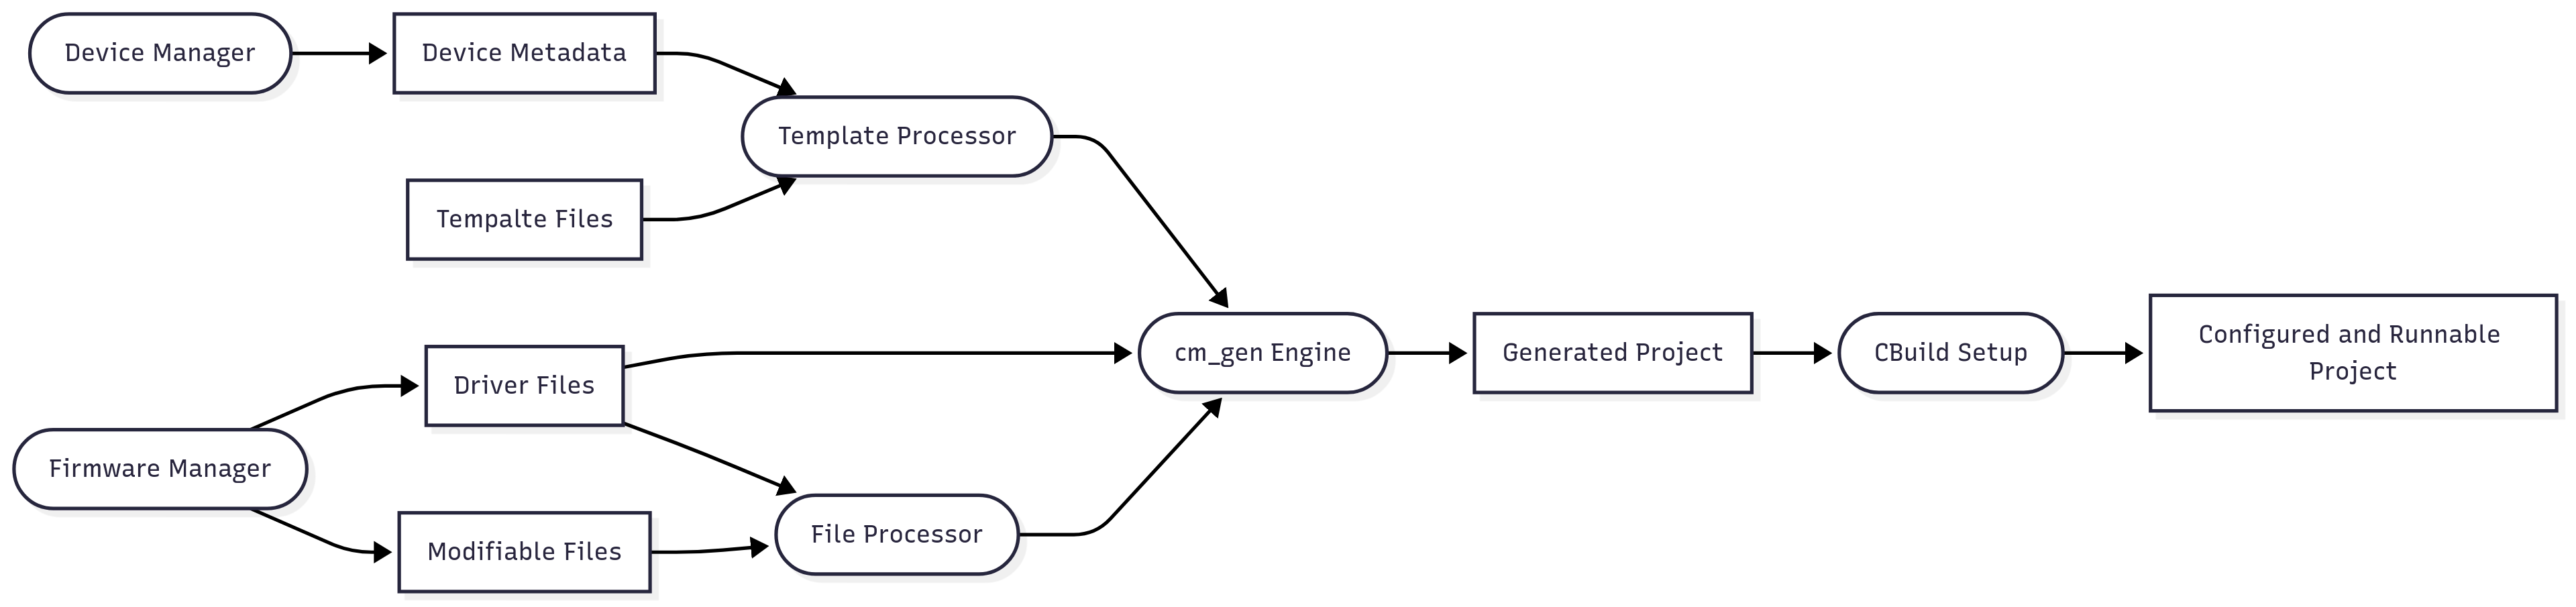
\includegraphics[width=15cm]{ST_Summer_Internship/GenerationToolComponents.png}
    \caption{Project Generation Tool Architecture}
    \label{fig:gen_tool_arch}
\end{figure}

\section{Use-Case Diagram}
\begin{figure}[H]
  \centering
  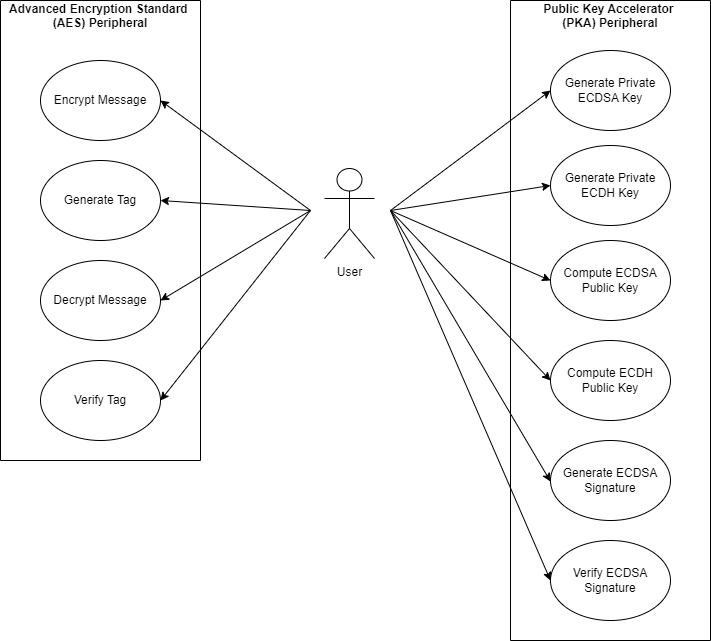
\includegraphics[width=14.5cm]{img/use case 2.png}
  \caption{Use-Case Diagram for Cryptographic Peripherals (AES and PKA)}
  \label{fig:use_case_diagram}
\end{figure}

The Use-Case diagram in Figure \ref{fig:use_case_diagram} illustrates the interactions between a user and the cryptographic peripherals available on STM32 MCUs.
 Refer to Table \ref{tab:use_cases} for an in-depth explanation:

\begin{longtable}{|p{5cm}|p{6cm}|p{4cm}|}
\caption{Use Cases for Cryptographic Peripherals} \label{tab:use_cases} \\

\hline
\textbf{Use Case} & \textbf{Relevance} & \textbf{Peripheral Used} \\ \hline
\endfirsthead

\multicolumn{3}{c}%
{{\bfseries \tablename\ \thetable{} -- continued from previous page}} \\
\hline
\textbf{Use Case} & \textbf{Relevance} & \textbf{Peripheral Used} \\ \hline
\endhead

\hline \multicolumn{3}{|r|}{{Continued on next page}} \\ \hline
\endfoot

\hline
\endlastfoot

Generate Private ECDSA Key & Part of the key management process, ensuring secure storage and handling of private keys, which contributes to confidentiality. & PKA (Public Key Accelerator) \\ \hline
Generate Private ECDH Key & Part of the key management process and essential for establishing a shared secret, contributing to confidentiality. & PKA (Public Key Accelerator) \\ \hline
Compute ECDSA Public Key & Necessary for signature verification, which ensures authenticity. & PKA (Public Key Accelerator) \\ \hline
Compute ECDH Public Key & Necessary for the ECDH key exchange process, contributing to confidentiality. & PKA (Public Key Accelerator) \\ \hline
Generate ECDSA Signature & Ensures the authenticity of the communicating parties by providing a way to verify identities. & PKA (Public Key Accelerator) \\ \hline
Verify ECDSA Signature & Ensures the authenticity of the communicating parties by verifying the provided signatures. & PKA (Public Key Accelerator) \\ \hline
Encrypt Message & Ensures confidentiality and integrity of the message during transmission. & AES (Advanced Encryption Standard) \\ \hline
Generate Tag & Ensures the integrity of the message and also serves as an authentication check. & AES (Advanced Encryption Standard) \\ \hline
Decrypt Message & Ensures confidentiality and integrity of the message during transmission. & AES (Advanced Encryption Standard) \\ \hline
Verify Tag & Ensures the integrity of the message and also serves as an authentication check. & AES (Advanced Encryption Standard) \\ \hline

\end{longtable}






\section{Work Environment}
In this section, we outline the hardware and software resources utilized during the internship project that were essential for the development, testing, and demonstration of the "CryptoEngine" peripheral.

\subsection{Hardware Resources}
\begin{itemize}
    \item \textbf{STM32XX MCU:} The STM32XX microcontroller unit (MCU) is the primary hardware platform used for implementing and testing the "CryptoEngine" peripheral. The STM32XX series offers advanced cryptographic features and peripherals, making it ideal for secure communication applications.
    \item \textbf{STM32U545 MCU:} The STM32U545 microcontroller unit is used for comparison and interoperability with the STM32XX MCU. This board utilizes the AES and PKA peripherals to perform cryptographic operations, enabling secure key exchange and encryption.
    \begin{figure}[H]
  \centering
  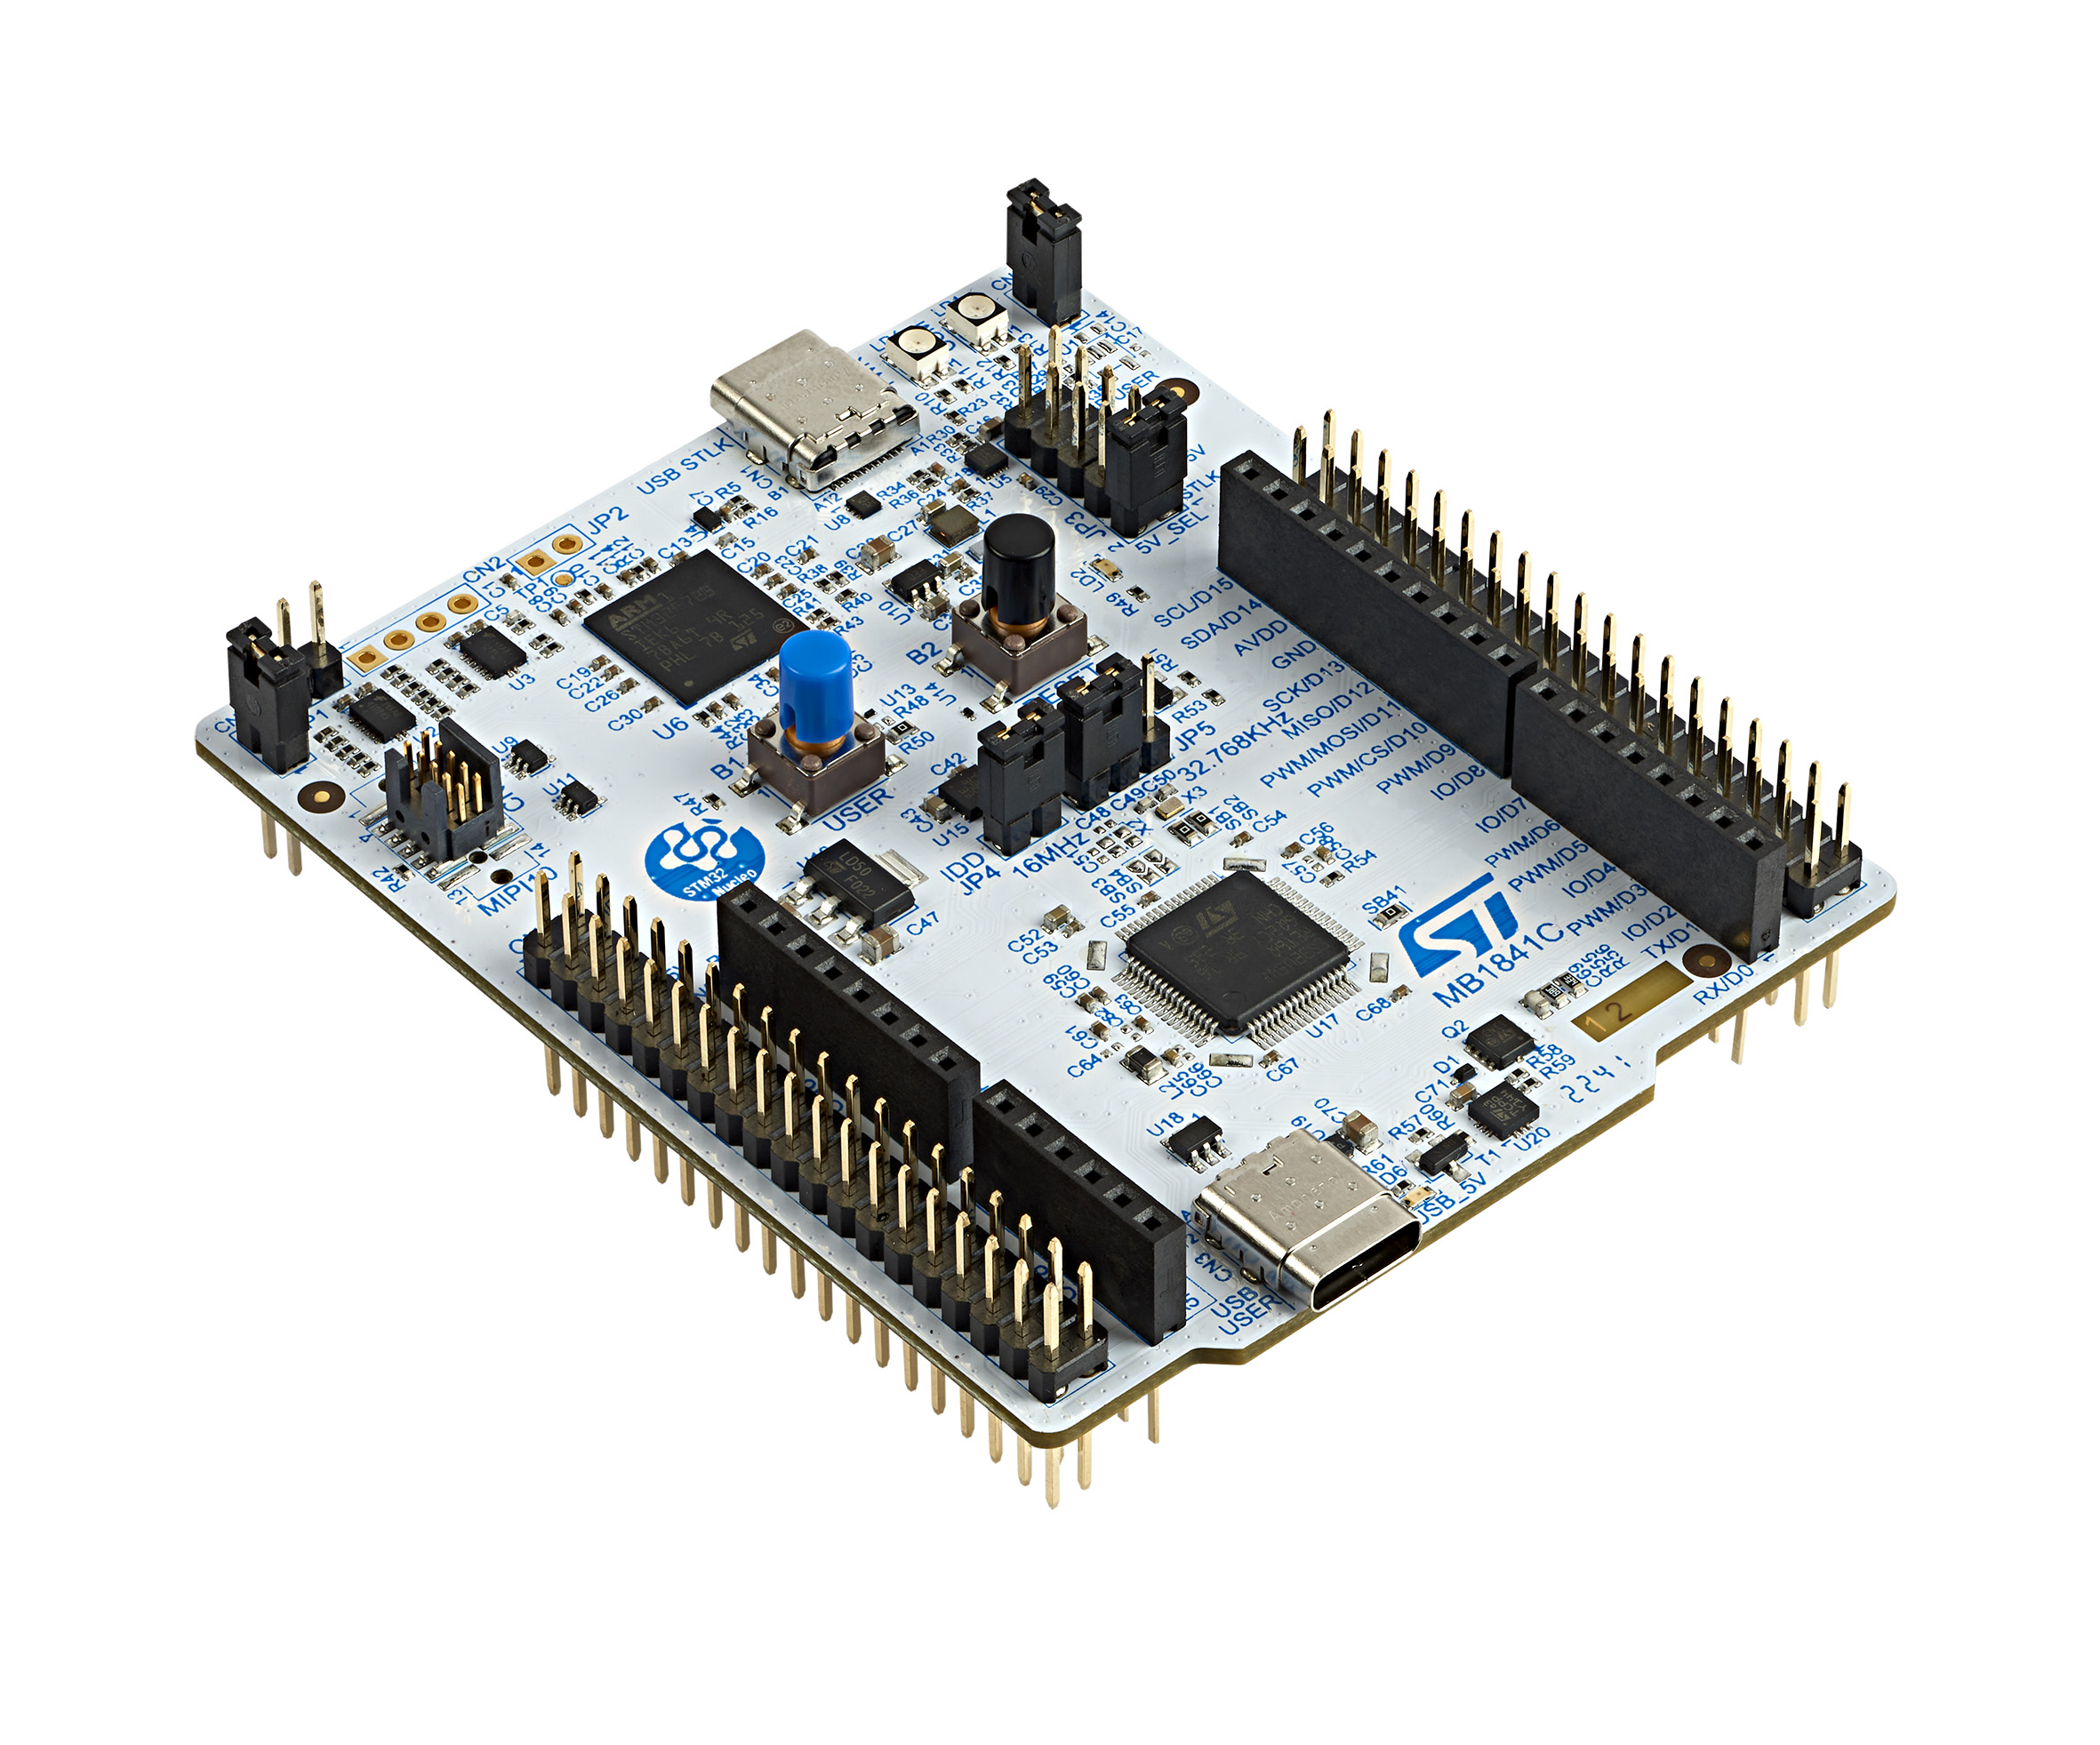
\includegraphics[width=6cm]{img/U5 Nucleo.jpg}
  \caption{STM32U545 Nucleo Board}
  \label{fig:stm32u545n}
\end{figure}
\end{itemize}

\subsection{Software Resources}
The following software tools were used for the  development, debugging and testing of the "CryptoEngine" demonstration:

\subsubsection{IAR Embedded Workbench}
IAR Embedded Workbench is an integrated development environment (IDE) used for programming, debugging, and optimizing embedded applications. It provides comprehensive support for STM32 microcontrollers, including the STM32XX and STM32U5 series. Key features include:
\begin{itemize}
    \item Advanced debugging capabilities with breakpoints, watch windows, and real-time data visualization.
    \item Code optimization tools to improve performance and reduce memory footprint.
    \item Integrated support for STM32CubeMX, allowing seamless project setup and configuration.
\end{itemize}
\begin{figure}[H]
  \centering
  
\includegraphics[width=8cm]{img/IAR.png}
  \caption{IAR Embedded Workbench}
  \label{fig:IAR}
\end{figure}

\subsubsection{STM32CubeMX}
STM32CubeMX is a graphical software configuration tool that simplifies the development of STM32-based applications. It allows developers to:
\begin{itemize}
    \item Configure microcontroller peripherals and middleware components through an intuitive graphical interface.
    \item Generate initialization code for STM32 microcontrollers, reducing development time.
    \item Integrate with various IDEs, including IAR Embedded Workbench, for a streamlined development workflow.
\end{itemize}
\begin{figure}[H]
  \centering
  
\includegraphics[width=8cm]{img/CUBEMX.jpg}
  \caption{STM32CubeMX}
  \label{fig:mx}
\end{figure}
\subsubsection{Yet Another Terminal (YAT)}
Yet Another Terminal (YAT) is a terminal application used for serial communication with the STM32 microcontrollers. It provides a user-friendly interface for monitoring and interacting with the microcontroller's output. Key features include:
\begin{itemize}
    \item Support for multiple communication protocols, including USART.
    \item Real-time data logging and visualization capabilities.
    \item Customizable settings for baud rate, data bits, parity, and stop bits.
\end{itemize}
\section*{Conclusion}
The work environment for this internship project includes both hardware and software resources that are essential for the successful implementation and demonstration of the "CryptoEngine" peripheral. The STM32XX MCU provides the necessary hardware capabilities, while the STM32U545 MCU is used for comparison and interoperability, utilizing AES and PKA peripherals. IAR Embedded Workbench and STM32CubeMX offer powerful tools for software development and configuration. Together, these resources enable the creation of a secure, efficient, and user-friendly cryptographic demonstration.
